\chapter{Science and Metrics}\label{Science and Metrics}

In 1955, Dr. Eugene Garfield published a fundamental paper in the history of bibliometric studies \cite{Garfield108}. In his work,
Garfield introduced the idea of a citation index, i.e., a database that would allow scientists to navigate the corpus of scientific publication through citation in order
to find valuable bibliographic material for their own research, an idea that eventually led to the foundation in 1960 of the Institute for Scientific Information (ISI).
While advocating for the importance of such index, Garfield used as an example the possibility to quantify the number of citations: \textit{"
Thus, in the case of a highly significant article, the citation index has a quantitative value, for it may help
the historian to measure the influence of the
article—that is, its ‘impact factor’"}, symbolically giving birth to the field of \textit{Scientometrics}, which
aims at providing a quantitative analysis of science and scientific research in general through statistical and mathematical analysis.
In 1972, Garfield
continued on this path by introducing a quantitative measure to rank journals based on their publication and citation count \cite{Garfield1972}. 

In its earliest
stages the field had a huge overlap with bibliometric and library studies in general, as well as with a quantitative analysis at a micro level, such as 
the individual habits of scientists \cite{069102832X}. With the increase of the availability of data scientometrics started to differentiate as its own
field aimed at the development of scientific indicators \cite{1208.4566}, also pushed by the increase need of instruments in the process of academic policy making 
\cite{doi:10.1080/09537329508524202}, with citation based measures being the dominating base in order to assess quality in scientific output. 
As more citation based analysis were being introduced \cite{Cole1972,vanRaan1993}, scientists also started to question the validity of such methods
to assess quality of research both from a technical point of view (i.e. the mathematical validity of the methods) as well as from a philosophical
one (do citations reflect quality?) \cite{ASI:ASI5,ASI:ASI7,MacRoberts1989,Seglen1997}.

In fact, the clash between the scientific requirement to cite relevant works along with the knowledge that metrics are used in order to assess
the quality of scientific research however, can lead to a vicious circle
in which the methods used to analyze the scientific outputs end up influencing the selection process of cited works \cite{HARGENS1990205}  or, in general, influencing the structure of 
Academia itself \cite{10.2307/765143}, thus compromising the previous underlying assumptions
of citations as a free and voluntary choice. In spite of these limitations, citation based metrics continued being introduced and citation based
rankings were introduced for authors \cite{10.2307/4152261} as well as for universities \cite{RankingUni}. In this chapter I will briefly go
through some of the most popular ranking measures for individual papers and authors.





\section{Publication rankings}
Even though a large of number of rankings for authors and journals were being developed, paper rankings required more time to be introduced.
Unlike metrics meant for groups of papers that allow to address the rankings statistically, ranking of papers comes down to the ranking
of individual nodes in a network. This task can be extremely challenging in the scientific network, especially considering
the difference in citation patterns across fields both quantitatively \cite{Radicchi11112008} and conceptually \cite{Franceschet2010}. Therefore
citation counts remained for a long time a valid ranking method locally, provided that one would know what the typical citation count
of a paper on a topic could be. 

In order to allow for a fair ranking across \textit{all} scientific publications instead, one would have to put into context the local properties of a paper, i.e.
 the community from which the citations come, with the global properties of the network, i.e. how the single community relates to all the others. This problem
 is closely related to what the well known Page Rank (PR) algorithm of Google does \cite{Page99thepagerank}. Page Rank was the most successful method among a number
 of solutions introduced in the 90s \cite{Kleinberg1999} for solving the problem of rating Web Pages in the WWW. Curiously, in their paper,
 Page and Brin analyze comparison between ranking pages and publications, concluding that citation counts are a far too limited tool in the presence
 of a large evolving network.
 
 The idea behind PR is to provide a metric for quality of web pages that takes into account the quality of the citations 
 themselves. In this framework therefore, a large degree (the equivalent of citation count) cannot be enough to receive a high PR as these citations
 might be incoming from poorly ranked nodes. In this framework therefore quality is built among a reinforcing behavior in which high quality pages
 "support" each other ranking wise through mutual citations or, in general, by being highly connected within the same community. Mathematically, the PR
 algorithm can be implemented in many ways, among which a recursive method that initially assigns equal ranking to all papers and then proceeds
 to propagate the ranking through the equation:
 \begin{equation} \label{eq:PR}
 PR(j) = \frac{1 -d }{N} + d \sum_{j \in N_{i}} \frac{PR(j)}{|N_{j}|} 
 \end{equation}
 where $N$ is the total number of nodes and $N_{i}$ is the neighborhood of node $i$. The PR can also be thus calculated by solving the eigenvalue equation $\vec{R} =  (1 -d)/N \vec{1} + d A\vec{R}$ where $\vec{R}$ is the array ranking and $A$ is the adjacency matrix of the WWW. The possibility 
 to express the PR algorithm in the solving of an eigenvalue equations shows that the PR is ultimately a centrality measure. The problem can be solved efficiently with the power method, requiring ~52 iterations to obtain convergence for the 
snapshot of the WWW that Page and Bring used in 1999 \cite{Page99thepagerank}.
The parameter $d$ is a quantity called \textit{damping factor} and it plays a crucial factor in the algorithm. The damping factor is linked to the
implementation of the model as a random walker that propagates the PR of a single node by randomly jumping
  to a nearby one through its links. In this context, the damping factor represents the probability for the walker to "get bored", as the authors say, and jump to a random
 node in the network after $1/d$ steps on average. Practically, this factor prevents the influence of "sinks" (node or group of nodes without outgoing links) that would absorb all 
 the rankings; with
 $d = 1$ we would have an infinite series of clicks, thus allowing the walker to be trapped in such sinks, while $d=0$ would be equal to a situation
 in which the PR are uniform and constant. However, the damping factor also plays a fundamental role in the correct renormalization of scores across communities
 of different sizes  \cite{Xie2007}. If a community is strongly isolated from the core of the network (i.e. it has few incoming links), it might be difficult
 for the random walker to enter the community and to correctly evaluate its global PR, without the necessity to perform separate rankings.
 
 This 
 feature of the Page Rank thus allows to solve issues linked to different topological structures of scientific communities in citation networks both across fields and within fields \cite{Maslov2008}.
 In 2007 two papers attempted two adapt the Page Rank algorithm to scientific publications. Chen et al. applied the pure Page Rank algorithm to all 
 publications belonging to the Physical Review family of journals from 1893 to 2003, with a choice of $d=0.5$ as they believed it would better
 reflect the citation practices in science. Even though the PR was shown to be positively correlated with the citation count, as expected  \cite{Fortunato:2007:API:1422841.1422847},
 a few paper were shown to be significant outliers and were identified as being important "gems" in Physics. In the same years a follow up paper came that introduced
 the CiteRank algorithm \cite{Walker2007}: a generalization of the PR algorithm, in which the effects of aging into the Page Rank algorithm
 are taken into account. This was necessary as the PR has in intrinsic directionality based on the fact that papers
 cannot be cited by older ones, thus forcing the "flow" of the PR towards older entries. In the CR framework, the random walker starts from a \textit{recent} paper
 and recursively follows scientific papers selecting a link not randomly, but rather in a weighed process that penalizes older papers and therefore
 gives a stronger value to novelty.
 
In Publication IV we introduced a measure that we called \textit{persistent influence}. Despite appearing at first glance similar to PR methods, it is conceptually
very different. In our approach in fact, we reversed the flow of time and we turned a stochastic process into a deterministic one. While the PR methods
measure how likely a random walker is to land on a single node, we imagined a scenario in which the knowledge created in an article percolates through the network of articles.
In this framework citing papers do not pass their own credit to the cited papers, but rather inherits it \textit{from} them.
Mathematically, we start from an original seed $s$ with an initial influence $I_s=1$ and we allow newer papers to inherit the influence
through the equation :
\begin{equation} \label{eq:impact}
 I_{j} = \sum_{i \in N_{j}}  \frac{I_{i}}{ k_{j}^{in}}
\end{equation}
where $ k_{j}^{in}$ is the in-degree (or, number of references) of the article $j$, and $N_j$ is the set of out-neighbors. The normalization guarantees that the total influence
that the cited articles have on article $j$ is 
constant and that the influence value does not exceed $1$.
As the process continues, the influence values dilute through the network, but at the same time they are spread to increasing number of articles. At the end of the process
we can then proceed to observe the influence that a single paper has had on the whole scientific network as shown in Fig.\ref{fig:influence}.





 \begin{figure}[h]
\centering
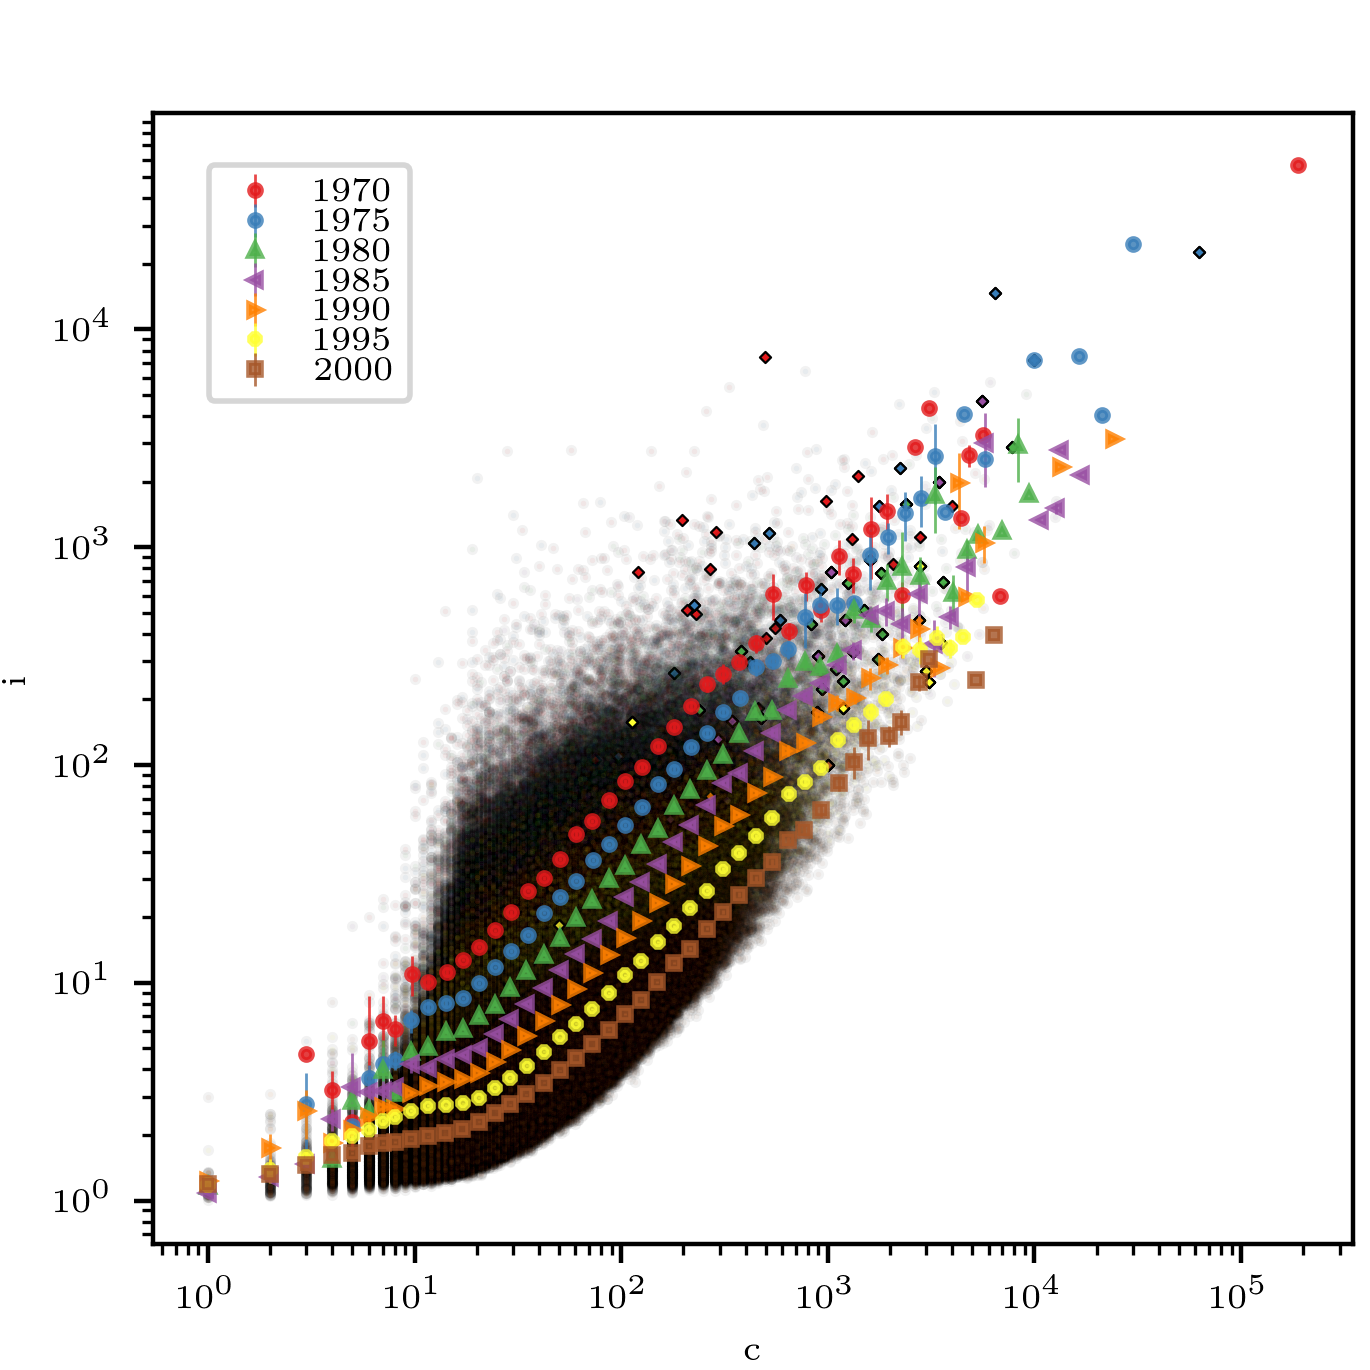
\includegraphics[width=.8\textwidth]{impact_thesis.png}%
\caption{Scatter plot of values for citations vs persistent influence for different years. The full dots represent the average influence for publications within the same citation
bin. Diamond shaped dots represent individual Nobel prize winning papers, the coloring of which is assigned according to the closest year to the publication date. The values appear to be correlated by a power law curve, but within
each citation bin influence values can span multiple orders of magnitude. Also, Nobel prize winning papers are clustered in the top right corner, indicating
both a high citation count and high influence values. Figure adapted from publication IV.}
\label{fig:influence}
\end{figure}


\section{Author rankings}

Science has primarily been a public endeavor carried out in public universities. 
As more investments were being
put into research, it is no surprise that soon pressure to properly quantify scientific output would start to increase \cite{Lane2011}.
Citation counts served this purposes and have been used to decide how to allocate funds \cite{Bornmann2005} as well as to select candidates for
academic positions \cite{Boyack2003}. In this search for a "perfect" measure, one of the most important contributions was developed in 2005 by J.E. Hirsch \cite{10.2307/4152261},
who introduced for the first time a clear metric aimed at ranking scientists through their citation count.
The h-index is based on a very straightforward definition: an author has index $h$ if $h$ of their publications have gathered at least $h$ citations each and the remaining
papers have citations $\leq h$. 

The new metric became immediately popular among scientists and started being considered as a standard to which to compare standard bibliometric indicators  \cite{vanRaan2006}, both
thanks to its simplicity and its ability to "rescue from obscurity" scientists who had been heavily contributing in very specific fields \cite{Ball2005}. However,
the h index was also soon discussed from a methodological point of view as authors claimed that it was not a correct way to quantify a career. In particular, it was pointed
out that one can artificially alter one's index through self-citations \cite{PURVIS2006} and that
citations need to be weighed, as not all of them carry the same weight \cite{Wendl2007}. As other critiques followed, tackling the limitation of the h index in guaranteeing a fair
ranking of scientists, new methods appeared, trying to fix the structural limitations of the h-index: indexes focusing on high cited papers (g-index) \cite{Egghe2006}, indexes focusing
on the average citations of the papers that grant the h-index to an author (A and AR index) \cite{Jin2007}, indexes focusing on the different
volume of publications across authors (h-normalized index) \cite{Sidiropoulos2007}, indexes that take into account the difference in lengths in careers (m-quotient) \cite{Burrell2007},
indexes that focus only on the most cited papers (Google Scholar's \textit{i10} index) \cite{i10} and many others \cite{Alonso2009}.

As citation based indexes continued to proliferate however, another key aspect became important to tackle: what is the predictive power of the h index? Since these measures
were being actively used as proxies of scientific excellence in the hiring process, it is normal to investigate the ability of the h index to predict the quality of individual
careers. Hirsch himself soon tackled the aspect, reporting that the h index is able to predict a carreer: \textit{"That is, a researcher with a high h index after 12 years is highly
likely to have a high h index after $24$ years"}\cite{Hirsch2007}.  
While more works have similar results by combining the h index with other citation based metrics \cite{Acuna2012}, other publications reported a different scenario in which
past citations are only good at predicting future citations to \textit{past} publications, but are ultimately not good at predicting future citations to \textit{future} publications \cite{Mazloumian2012}.
This contrast  between prediction of previous results vs prediction of past results brought back the attention to the
validity of the h index as a measure to predict the evolution of a career. In fact it has been argued that 
the h index suffers from methodological flaws due to the nature of its definition: the h index is a non stationary measure \cite{Penner2013b} which has a high auto correlation 
to its whole previous history, ultimately causing the h index being a good predictor of \textit{itself} \cite{Schreiber2013}. Quantitatively, any cumulative, non decreasing
measure has auto correlation between its index at two different stages of the career following the relation $Cor(h(t),h(t + \Delta t)) = \sqrt{\frac{t}{t + \Delta t}}$, which means
that the predictive power of such indexes is much lower when trying to estimate an individual's h-index many more years into their future than the current career
academic age ($t/(t + \Delta t) \rightarrow 0$) and that for the same prediction interval ($\Delta t$) the prediction will be much more sound for a senior researcher rather
than for a junior one \cite{Penner2013}. This latter result leads to the consequence that the h index of a researcher, as their career progresses, increases regardless
of their productivity \cite{Schreiber2013}. 

These findings are
 ultimately in contrast with the very idea that metrics should be used to hire someone for that they will do, since such kind of citation metrics based on previous results appear to be able
 grasp mainly only what a scientist has done and show their strongest predictive limitations for the cases in which these will be used in real academic hiring decisions \cite{Penner2013}. Furthermore,
 it can even introduce a self-reassurance bias as bureaucrats may actually take advantage of the metric auto correlation in order to have a guarantee that metrics will increase \cite{Schreiber2013}.

 In parallel to citation based rankings however, other authors have attempted to introduce rankings based on methods similar to the Page Rank algorithm discussed in the previous paragraph \cite{PhysRevE.80.056103,Yan2010}
as well as on centrality measures similar to the one mentioned in section \ref{sec:centrality} \cite{Yan2009}, but ultimately the intrinsic feasibility of the distinction
between quality and quantity in scientific output is still an open question \cite{Kaur2015} and the predictability of individual indexes remains a statistical method that can possibly
lead to average results, while careers have been shown to be extremely uncertain and volatile, with single events leading both to sudden career boosts \cite{10.1371/journal.pone.0018975} and negative shocks
to equally extreme, yet opposite consequences \cite{Petersen2012}. Even though it is probably impossible to either develop a perfectly universal and unbiased metrics or to
prevent the usage of metrics in the academic selection process, it has been argued that it would be most beneficial to minimize the increasing ``taste for publication'' \cite{Osterloh2010}
that has been gradually replacing the "taste for science" and to rely on multiple factors and measure instead of reducing the process to the evaluation of a 
single statistic \cite{Frey2010}.